\documentclass{article}
\usepackage{tikz}
\usepackage{amsmath}  
\usepackage{amssymb} 
\usepackage[a4paper]{geometry}
\usepackage{fancyhdr}
\pagestyle{fancy}
\lhead{Wachstum}
\rhead{März 2025}
\begin{document} 
\section{Wachstumsfunktionen}
Wachstumsfunktionen beschreiben zeitlich einen kontextuellen Bestand und dessen Wachstum. Die Limits der Funktionen sind anhand der Graphen und etwas Intuition der Funktionstermen gegenüber offensichtlich.
\subsection{Exponentielles Wachstum}
Exponentielles Wachstums beschreibt ein Wachstum, welches durch eine Exponentialfunktion modelliert werden kann. Dabei ist die momentane Wachstumsgeschwindigkeit zum Bestang proportional, sodass der Funktionswert mit der Zeit, desto höher der Bestand bereits ist, schneller ansteigt.
 
\noindent \begin{minipage}{5cm}
  \centering
  \begin{tikzpicture}     
    \draw[->, blue, thick, domain=-2:1.3, samples=50] 
              plot (\x, {e^(\x)});
       
    \draw[->] (-2, 0) -- (2, 0); 
    \draw[->] (0, -0.5) -- (0, e^1.3);
   
    \draw (0, 0) node[below left] {0};    
  \end{tikzpicture}
\end{minipage}
\hfill
\begin{minipage}{\dimexpr\textwidth-5cm}
Mit dem Anfangsbestand $f(0)=A$, dem Wachstumsfaktor $b$ und bei Bedarf der Wachstumskonstante $k=\ln{b}$ gilt
\[ 
 A \cdot b^x 
 \quad \text{oder} \quad 
 A \cdot \mathrm{e}^{k \cdot x}  
\] 
Solange ${b > 1 \implies k > 0}$ ist die Funktion streng monoton steigend. Bei einer prozentualen Steigung von $s$ pro Zeiteinheit ist ${b=1+s}$, wobei $s$ als Dezimalzahl ausgedrückt wird. Daraus kann dann auch $k$ bestimmt werden. \newline
Liegt beispielsweise eine Steigung um $15\%$ pro Zeiteinheit vor, ist ${b=1 + 0,15=1,15 \implies k=\ln{1,15} \approx 0,14}$. 
\end{minipage}
Es gilt $f'(x) = k \cdot f(x)$, woraus offensichtlich wird, dass die Steigung, die Wachstumsgeschwindigkeit, vom zurzeitigen Bestand abhängig ist.
 
\subsubsection{Exponentieller Zerfall}
\begin{minipage}{\dimexpr\textwidth-5cm}
Ist hingegen das ${b < 1 \implies k < 0}$, fällt die Funktion streng monoton und es liegt ein exponentieller Zerfall vor. $b$ und $k$ ist nun jeweils der Abnahmefaktor und die Zerfallskonstante. Bei gegebener prozentualer Zerfallsrate pro Zeiteinheit ist ähnlich wie oben vorzugehen, nur mit einer Subtraktion anstelle von einer Addition zu $1$, also gilt ${b=1-s}$. \newline
Liegt beispielsweise eine Verlust von $15\%$ pro Zeiteinheit vor, ist ${b=1-0,15=0,85 \implies k=\ln {0,85} \approx -0,16}$. 
\end{minipage}
\hfill
\begin{minipage}{5cm} 
 \centering
  \begin{tikzpicture}     
    \draw[->, blue, thick, domain=-ln(3):2, samples=50] 
              plot (\x, {e^(-\x)});
       
    \draw[->] (-2, 0) -- (2, 0); 
    \draw[->] (0, -0.5) -- (0, 3);
   
    \draw (0, 0) node[below left] {0};    
  \end{tikzpicture}
\end{minipage} 
 
\subsection{Begrenztes Wachstum}
\begin{minipage}{5cm} 
  \centering
  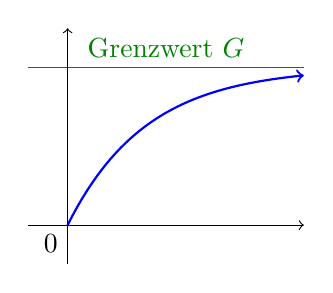
\begin{tikzpicture}     
    \draw[->, blue, thick, domain=0:3, samples=50] 
              plot (\x, {(0-2) * e^-\x + 2});
    
    \draw[green!50!black] (-0.5, 2) -- (3, 2) node [midway, above] {Grenzwert $G$}; 
 
    \draw[->] (-0.5, 0) -- (3, 0); 
    \draw[->] (0, -0.5) -- (0, 2.5);
   
    \draw (0, 0) node[below left] {0};    
  \end{tikzpicture}
\end{minipage}
\hfill
\begin{minipage}{\dimexpr\textwidth-5cm} 
Begrenztes Wachstum beginnt bei einem Anfangsbestand $A$ bevor es sich anfangs schnell an den Grenzwert $G$ nähert. Die Steigung geht dabei, desto näher der Bestand an der Grenze ist, zu null. Es gilt
\[
 f(x) = (A-G) \cdot e^{-kx} + G 
\]
mit der DGL
\[
 f'(x) = k \cdot (G - f(x)) 
\]
\end{minipage}
 
\vspace{1em} 
\noindent Beider dieser Formeln können sehr intuitiv interpretiert werden 
\begin{description}
 \item[Funktionsgleichung] Zu beginn wird der Graph um $A-G$, der Differenz zwischen dem Anfangsbestand und dem Grenzwert, also der Distanz, welche der Graph im verlauf der Kurve steigen muss, nach unten verschoben. Dies wird mit dem exponentiellen Zerfall $e^{-kx}$, welcher somit bei $f(0)=1$ beginnt und zu $0$ sinkt, multipliziert. Somit fängt der Graph bei $A-G$ an, bis er zu $0$ geht. Wird nun $+G$ addiert, geht der Graph von $A$ zu $G$.
 \item[Differenzialgleichung] Zu jedem Zeitpunkt ist die Steigung des Graphes zu der noch zu überquerenden Strecke, der Differenz zwischen $G$ und $f(x)$, mit dem Faktor $k$ proportional.
\end{description} 
\subsubsection{Schulbuchschreibweise}
Das begrenzte Wachstum kann auch als
\[
 f(x) = S-c \cdot e^{-kt}
 \quad \text{und} \quad
 f'(x) = k \cdot (S - f(x)) 
\]
aufgeschrieben werden, wobei weil $f(0) = S - c \cdot 1 \implies c = S - f(0)$ und S die Grenze ist. 
 
\subsection{Logistisches Wachstum} 
\begin{minipage}{6cm}
  \centering
  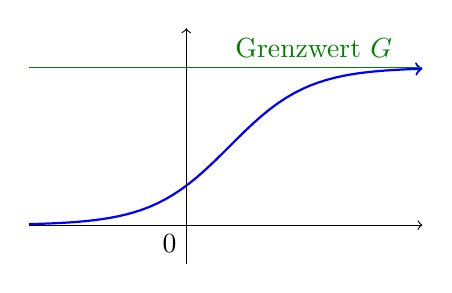
\begin{tikzpicture}     
    \draw[->, blue, thick, domain=-2:3, samples=50] 
              plot (\x, {(0.5*2)/(0.5+(2-0.5)*e^(-2*\x))});
    
    \draw[green!50!black] (-2, 2) -- (3, 2) node [midway, above right] {Grenzwert $G$};
 
    \draw[->] (-2, 0) -- (3, 0); 
    \draw[->] (0, -0.5) -- (0, 2.5);
   
    \draw (0, 0) node[below left] {0};    
  \end{tikzpicture}
\end{minipage}
\hfill
\begin{minipage}{\dimexpr\textwidth-6cm}  
Logistisches Wachstum beschreibt Wachstum, welches zuerst bei $f(0)=A$ exponentiell beginnt, bevor es auf die Grenze $G$ trifft.
Die generelle Formel ist
\[
 f(x) = \frac{A \cdot G}{A+(G-A) \cdot e^{-kGx}}
\]
mit der DGL
\[
 f'(x) = k \cdot f(x) \cdot (G-f(x))
\]
\end{minipage}
 
\vspace{\baselineskip} \noindent  
Die DGL zeigt, dass die Wachstumsgeschwindigkeit eines logistischen Wachstums sowohl von dem momentanen Bestand als auch von der Differenz zur grenze abhängig ist.
 
\subsubsection{Schulbuchschreibweise}
Im Schulbuch wird das Logistische Wachstum als 
\[
 f(x) = \frac{S}{1 + c \cdot e^{-kSx}}
 \quad \text{und} \quad
 f'(x) = k \cdot f(x) \cdot (S-f(x)) 
\]
aufgeschrieben, wieder mit S als Grenze, diesmal aber mit $c = \dfrac{S}{f(0)}-1$.
 
\subsection{Wachstumsgeschwindigkeiten}
Für jede Funktion, die ein exponentielles Wachstum beschreibt, $f(x)$, beschreibt die erste Ableitung $f'(x)$ die Wachstumsgeschwindigkeit. \newline
Gegenteilig ist die Stammfunktion von der Ableitung der Bestandsfunktion die Bestandsfunktion selbst, sodass die Änderung des Bestandes als bestimmtes Integral der Wachstumsgeschwindigkeit angesehen werden kann. Beschreibt $f(x)$ die Wachstumsgeschwindigkeit, so stellt
\[
 \int_{t_1}^{t_2} f(x) \,\mathrm{d}x 
\]
die Änderung des Bestandes zwischen den Zeitpunkten $t_1$ und $t_2$ dar. 
 
\end{document} 
 
 
 
 
